%%%%%%%%%%%%%%%%%%%%%%%%%%%%%%%%%%%%%%%%%%%%%%%%%%%%%%%%%%%%%%%%%%%%%%%%%%%%%%%

\section*{\large Exercício 1}
\addcontentsline{toc}{chapter}{\protect\numberline{}\large Exercício 1}%

Neste exercício são graficados diferentes chirps e seus espectros de Fourier. Chirps são funções contínuas que podem representar sinais com as características de frequência crescente (\textit{chirp-up}) ou descrescente (\textit{chirp-down}) no tempo. Quatro chirps diferentes são aqui estudados: chirp gaussiano, linear, quadrático (ou square) e hiperbólico. Eles são explorados no contexto da Análise de Fourier. %e, em particular, da transformada janelada de Fourier (ou WFT, do inglês Windowed Fourier Trnasform) e do espectrograma.

A função de densidade espectral para esse exercício foi assim definida:
\lstinputlisting[language=python, style=mystyle, firstline=12, lastline=30]{../scripts/exercicio1/chirp_psd.py}

%Bla bla bla

%\lstinputlisting[language=python, style=mystyle, firstline=36, lastline=48]{f90_integral_paralelo.f90}\\


%\begin{lstlisting}[language=bash,style=mystyle2]
%Somatorio de C:  1.9609359E+20

%real	0m0.219s
%user	0m0.212s
%sys	0m0.006s
%\end{lstlisting}


\subsection*{1.1} 
\addcontentsline{toc}{section}{\protect\numberline{} 1.1}%
Definição da função \textbf{chirp gaussiano}:
\lstinputlisting[language=python, style=mystyle, firstline=34, lastline=35]{../scripts/exercicio1/chirp_psd.py}

Gerando sinal chirp e seu espectro (variável global \texttt{N} também é usada na definição dos demais sinais):
\lstinputlisting[language=python, style=mystyle, firstline=48, lastline=56]{../scripts/exercicio1/chirp_psd.py}

\subsection*{1.2}
\addcontentsline{toc}{section}{\protect\numberline{} 1.2}%
Definição da função \textbf{chirp linear}:
\lstinputlisting[language=python, style=mystyle, firstline=37, lastline=38]{../scripts/exercicio1/chirp_psd.py}

Gerando sinal chirp e seu espectro:
\lstinputlisting[language=python, style=mystyle, firstline=58, lastline=64]{../scripts/exercicio1/chirp_psd.py}

\subsection*{1.3} 
\addcontentsline{toc}{section}{\protect\numberline{} 1.1}%
Definição da função \textbf{chirp quadrático} ou square:
\lstinputlisting[language=python, style=mystyle, firstline=40, lastline=41]{../scripts/exercicio1/chirp_psd.py}

Gerando sinal chirp e seu espectro:
\lstinputlisting[language=python, style=mystyle, firstline=66, lastline=72]{../scripts/exercicio1/chirp_psd.py}

\subsection*{1.4}
\addcontentsline{toc}{section}{\protect\numberline{} 1.2}%
Definição da função \textbf{chirp hiperbólico}:
\lstinputlisting[language=python, style=mystyle, firstline=43, lastline=44]{../scripts/exercicio1/chirp_psd.py}

Gerando sinal chirp e seu espectro:
\lstinputlisting[language=python, style=mystyle, firstline=74, lastline=80]{../scripts/exercicio1/chirp_psd.py}

A Figura com os chirps e seus espectros foi assim gerada (Figura 1.1):

\lstinputlisting[language=python, style=mystyle, firstline=84, lastline=128]{../scripts/exercicio1/chirp_psd.py}

% FIGURA
\begin{figure}[ht!]
	\legenda{Figura 1.1: Sinais chirp do Exercício 1 e seus respectivos espectros de potência calculados via FFT. As partes reais (linhas cheias em vermelho) e imaginárias (linhas tracejadas em azul) dos chirps são exibidas.}
	\vspace{1mm}	% acrescentar o espaçamento vertical apropriado entre o título e a borda superior da figura
	\begin{center}
		\resizebox{\textwidth}{!}{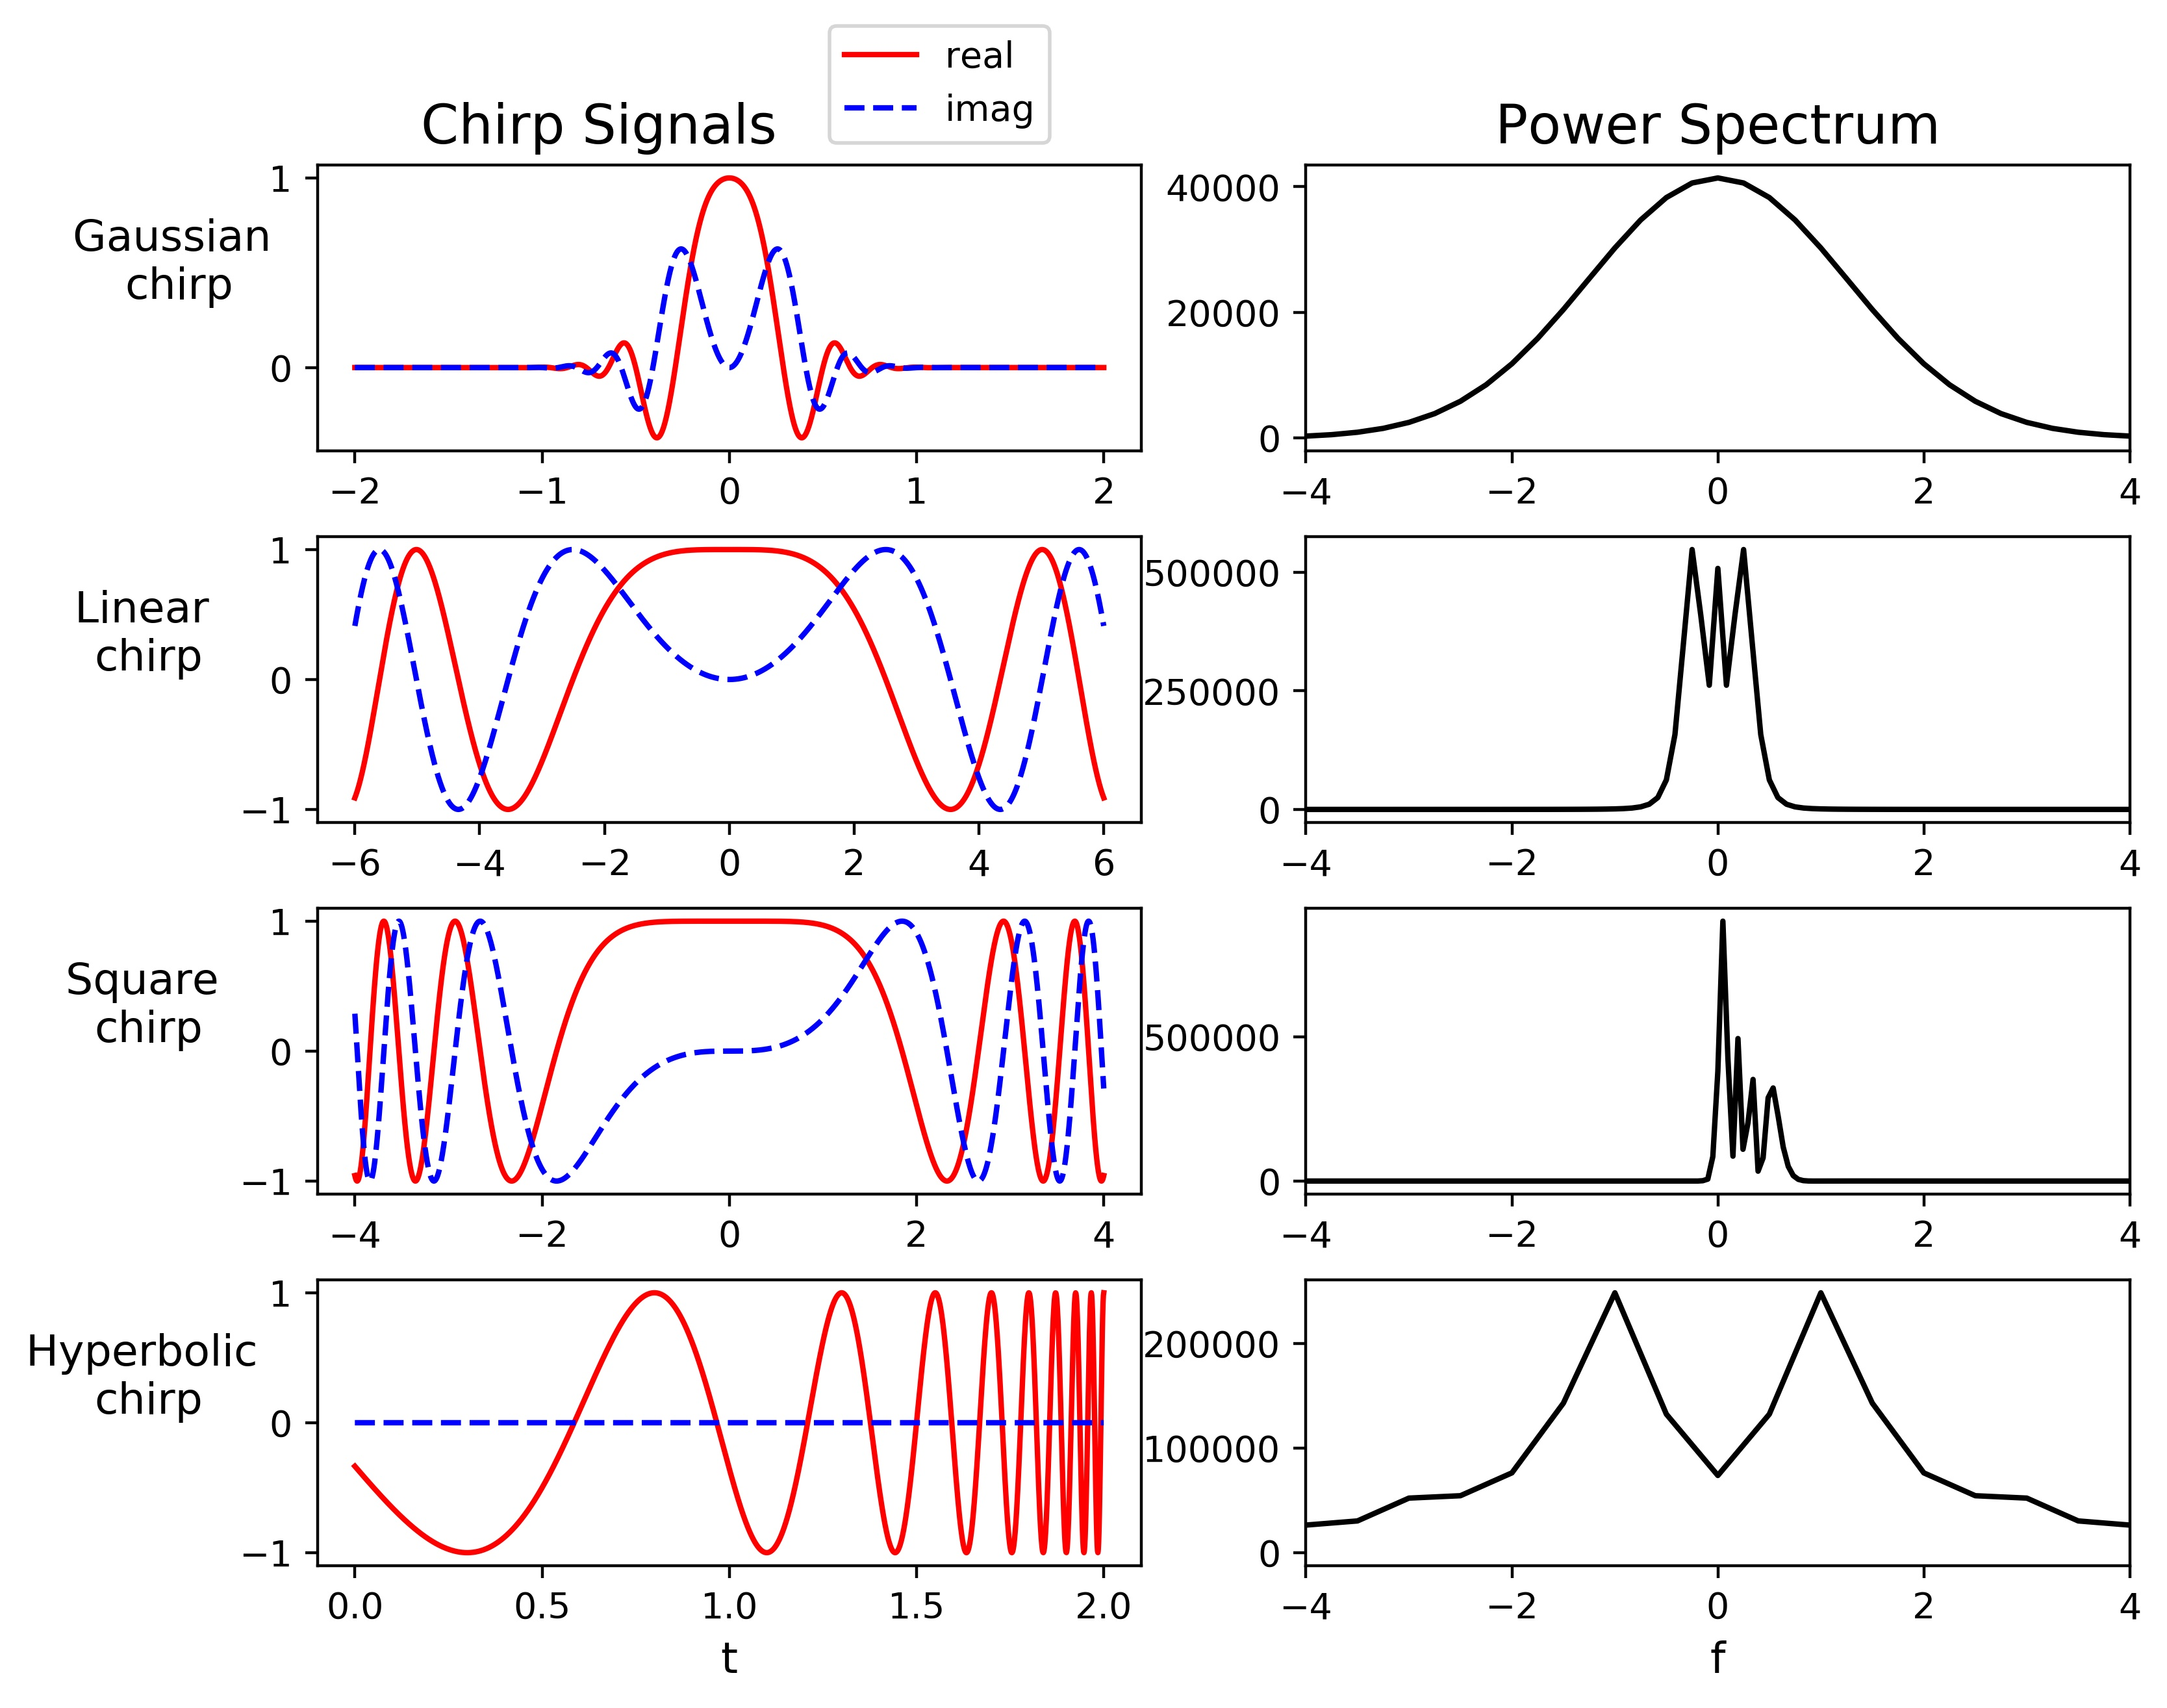
\includegraphics{../scripts/exercicio1/chirps_psd.jpg}}	
	\end{center}
	\vspace{-1mm}	% acrescentar o espaçamento vertical apropriado entre a borda inferior da figura e a legenda ou a fonte quando não há legenda (o valor pode ser negativo para subir)
	%\legenda{Figura 1.1: Dez sinais e seus respectivos histogramas para  asérie com $N$ = 64 do grupo noise.}	% legenda - para deixar sem legenda usar comando \legenda{} (nunca deve-se comentar o comando \legenda)
	\label{ex1_fig1}
	%\FONTE{}	% fonte consultada (elemento obrigatório, mesmo que seja produção do próprio autor)
\end{figure}

O código do início desta seção pode ser modificado (função \texttt{psd}) de modo que seu output  seja a Transformada de Fourier. O resultado é exibido na Figura 1.2. 

% FIGURA
\begin{figure}[ht!]
	\legenda{Figura 1.2: Sinais chirp e suas Transformadas de Fourier calculadas via FFT. As partes reais (linhas cheias em vermelho) e imaginárias (linhas tracejadas em azul) são exibidas.}
	\vspace{1mm}	% acrescentar o espaçamento vertical apropriado entre o título e a borda superior da figura
	\begin{center}
		\resizebox{\textwidth}{!}{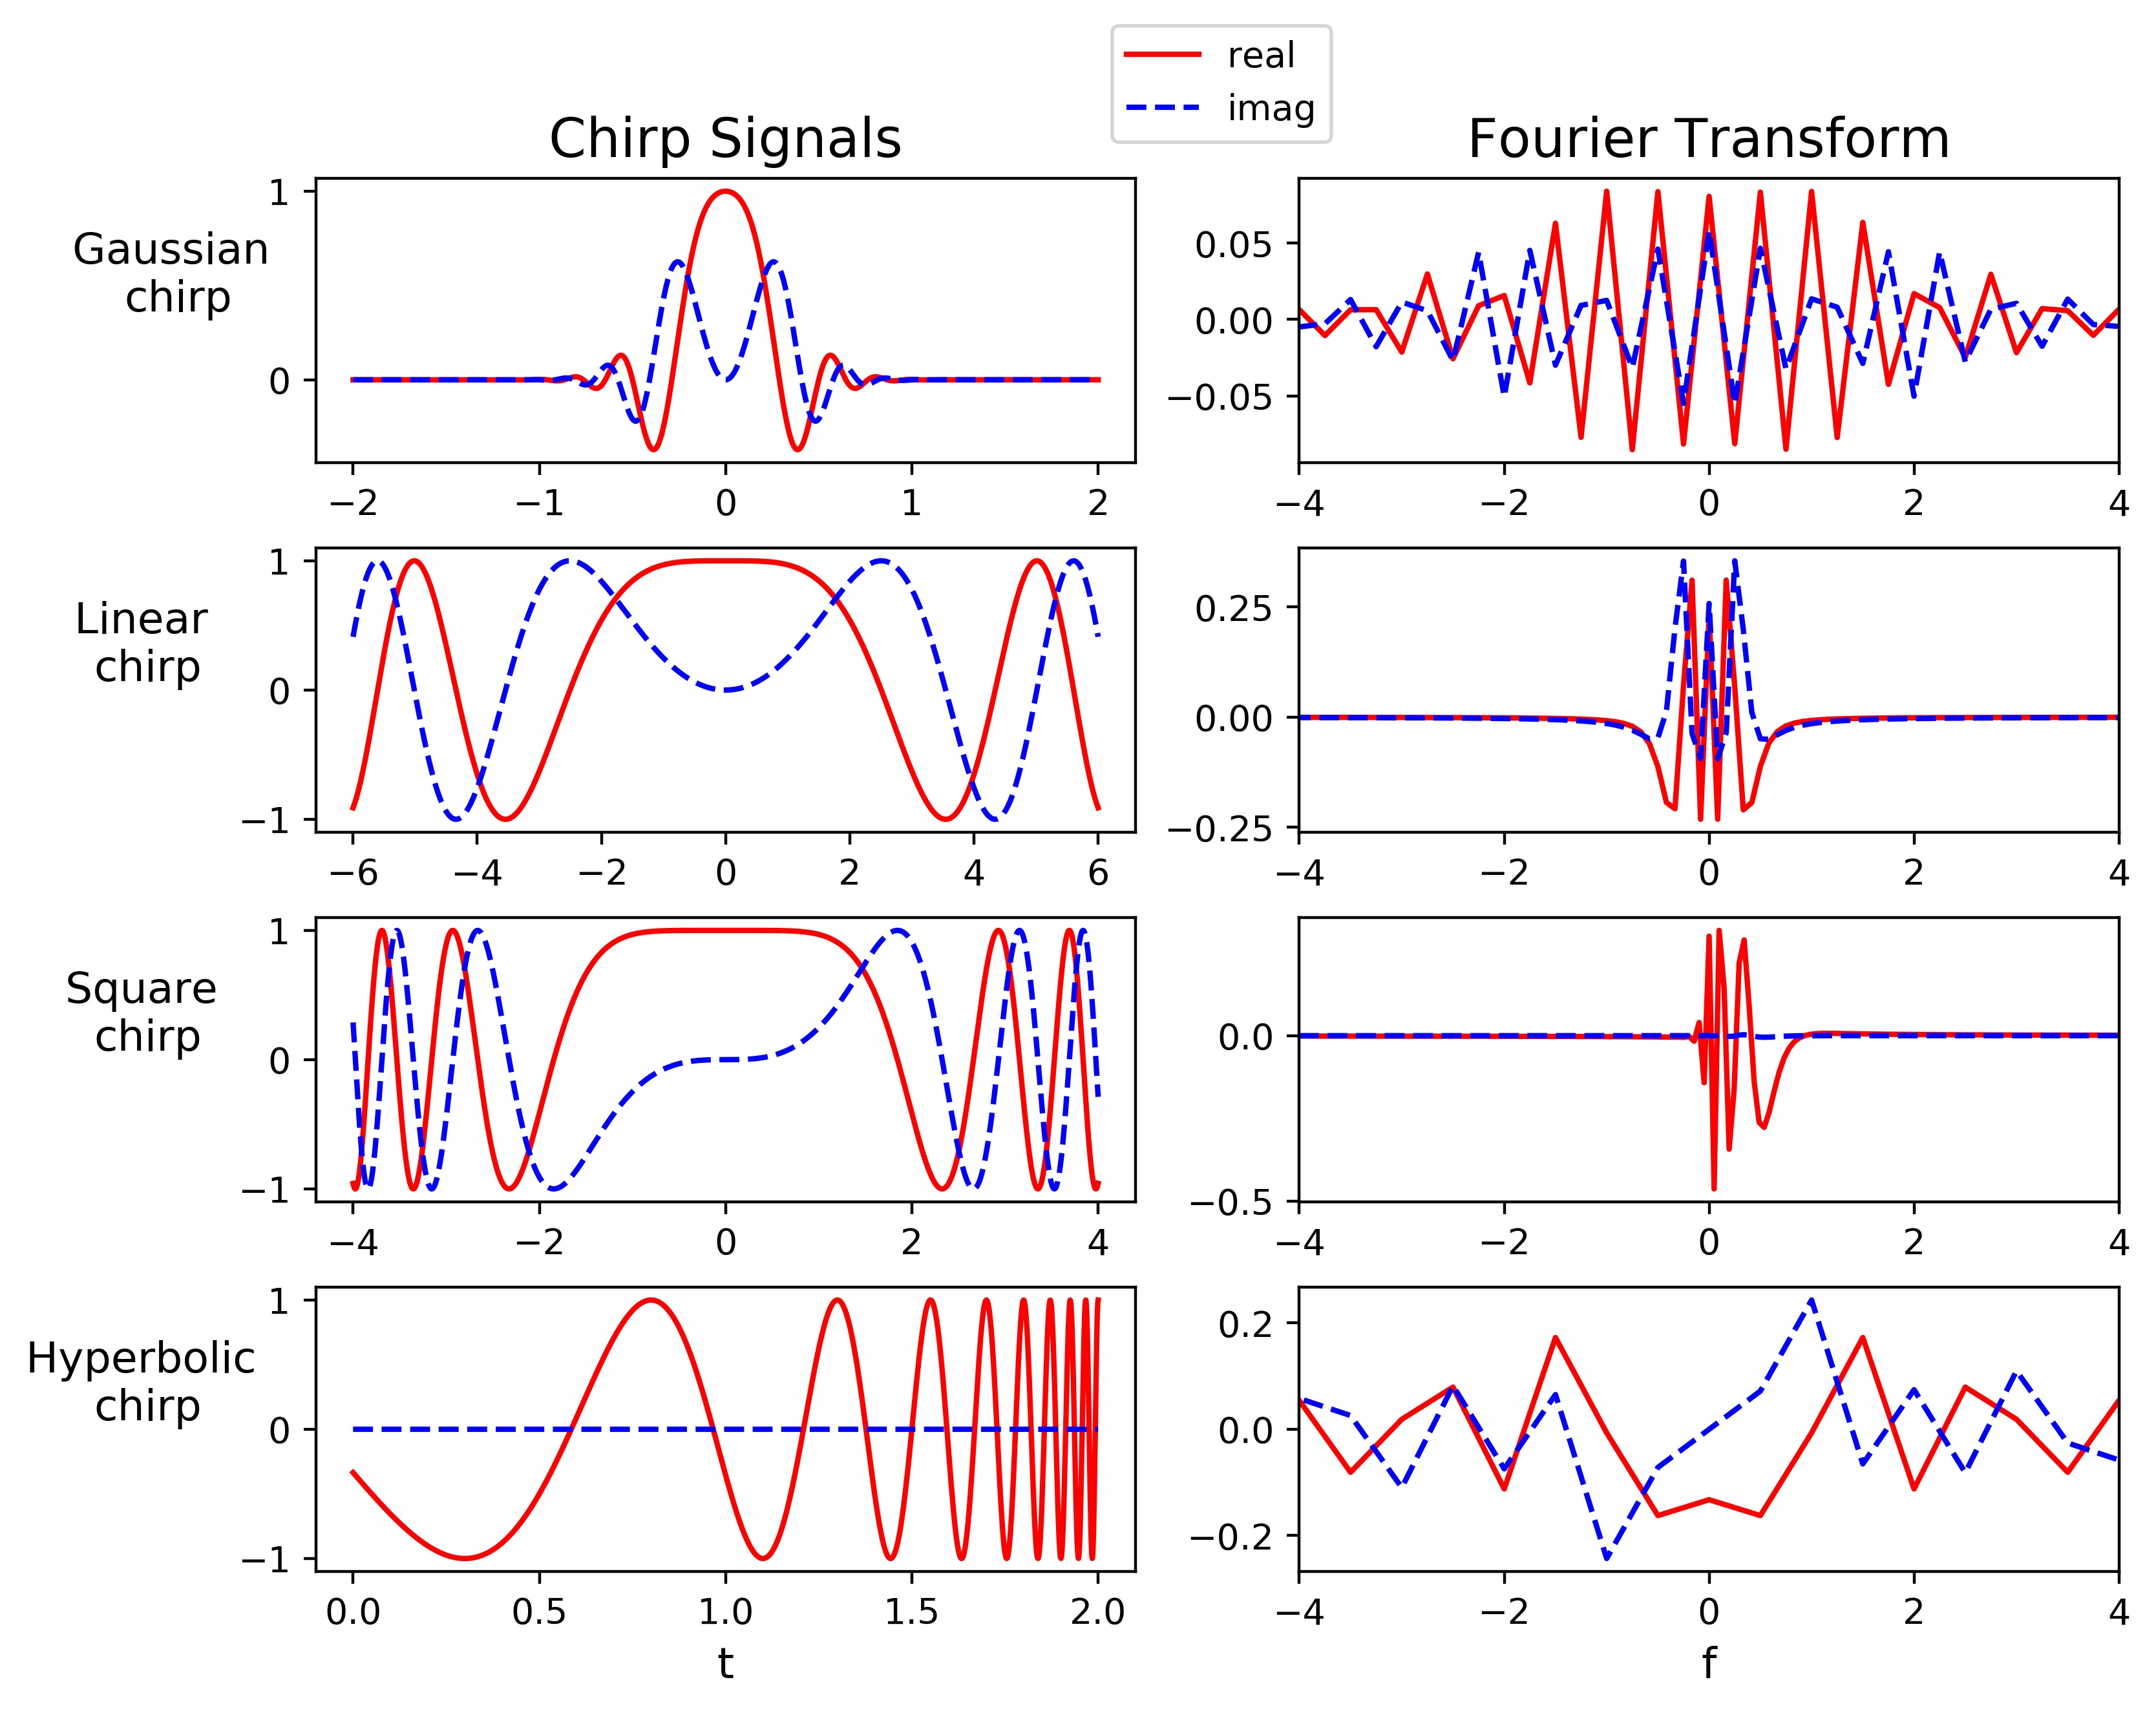
\includegraphics{../scripts/exercicio1/chirps_FT.jpg}}	
	\end{center}
	\vspace{-1mm}	% acrescentar o espaçamento vertical apropriado entre a borda inferior da figura e a legenda ou a fonte quando não há legenda (o valor pode ser negativo para subir)
	%\legenda{Figura 1.1: Dez sinais e seus respectivos histogramas para  asérie com $N$ = 64 do grupo noise.}	% legenda - para deixar sem legenda usar comando \legenda{} (nunca deve-se comentar o comando \legenda)
	\label{ex1_fig1}
	%\FONTE{}	% fonte consultada (elemento obrigatório, mesmo que seja produção do próprio autor)
\end{figure}


A Figura a seguir exibe o comportamento dos chirps e suas transformadas para o $t \in [0,6]$:

% FIGURA
\begin{figure}[ht!]
	\legenda{Figura 1.3: Sinais chirp do Exercício 1 e seus respectivos espectros de potência para o domínio $t \in [0,6]$.}
	\vspace{1mm}	% acrescentar o espaçamento vertical apropriado entre o título e a borda superior da figura
	\begin{center}
		\resizebox{\textwidth}{!}{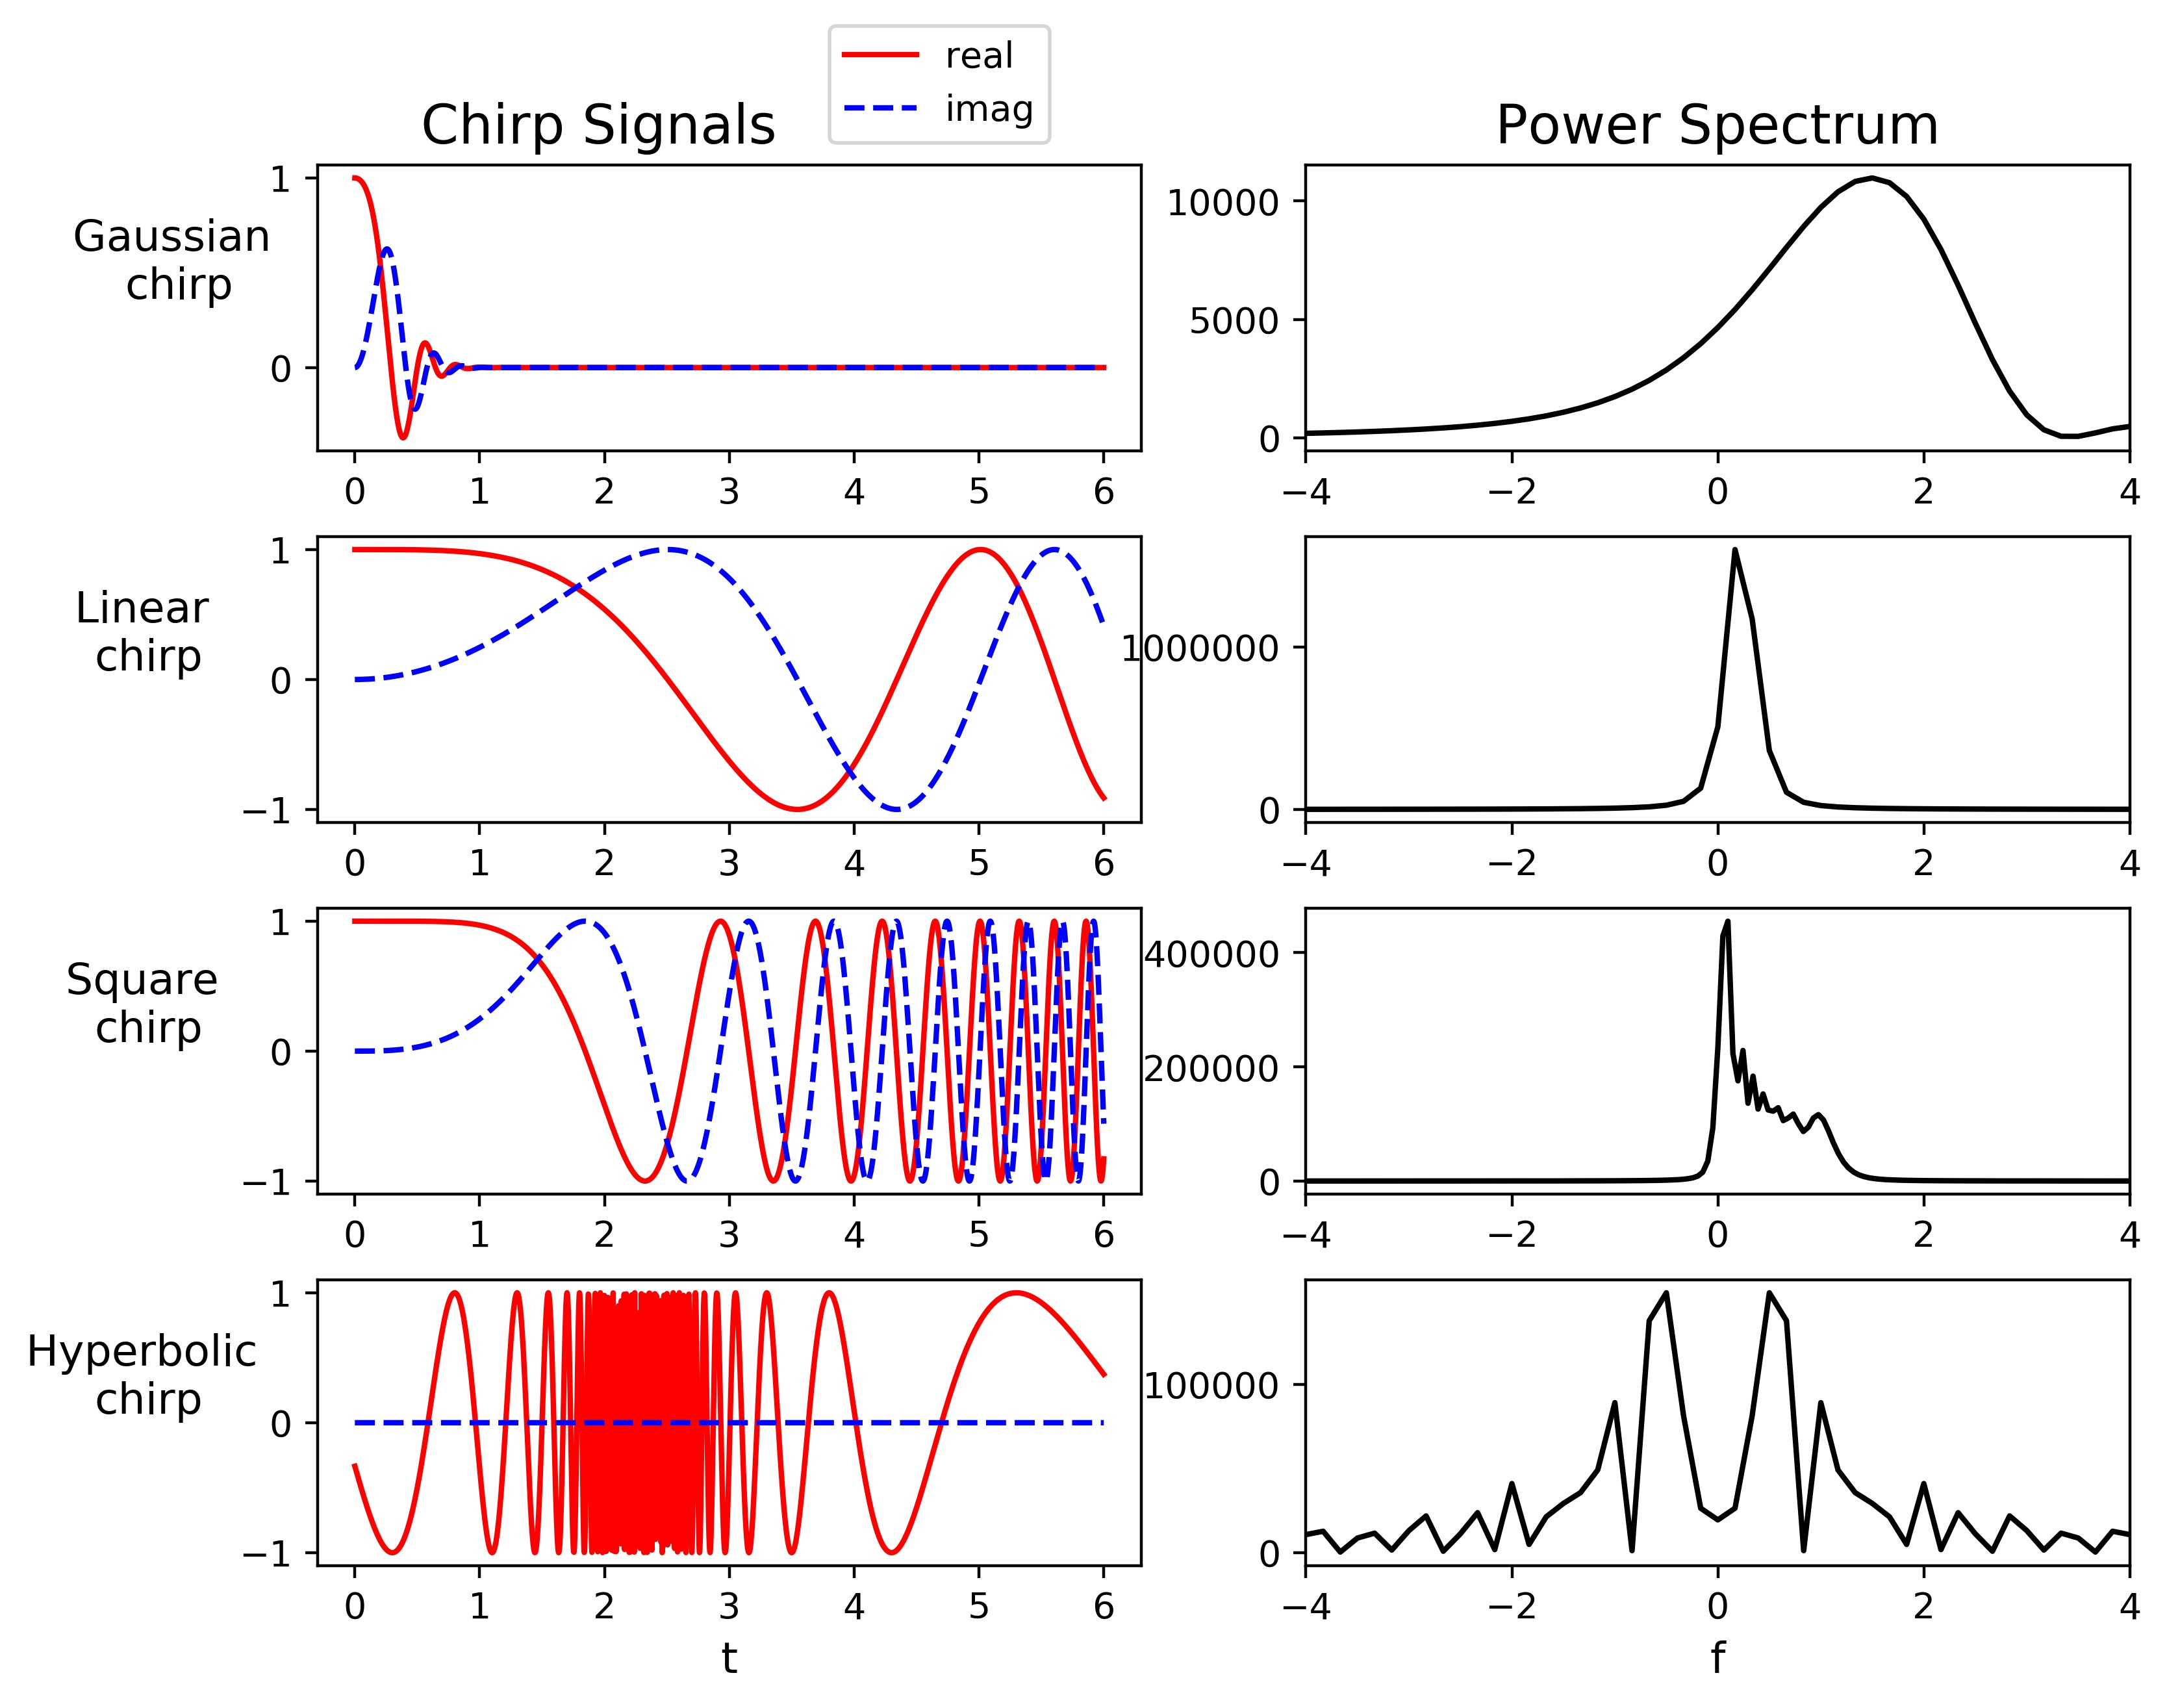
\includegraphics{../scripts/exercicio1/TEST_chirps_psd.jpg}}	
	\end{center}
	\vspace{-1mm}	% acrescentar o espaçamento vertical apropriado entre a borda inferior da figura e a legenda ou a fonte quando não há legenda (o valor pode ser negativo para subir)
	%\legenda{Figura 1.1: Dez sinais e seus respectivos histogramas para  asérie com $N$ = 64 do grupo noise.}	% legenda - para deixar sem legenda usar comando \legenda{} (nunca deve-se comentar o comando \legenda)
	\label{ex1_fig1}
	%\FONTE{}	% fonte consultada (elemento obrigatório, mesmo que seja produção do próprio autor)
\end{figure}


Conclui-se das Figuras 1.1, 1.2 e 1.3 que os chirps possuem uma natureza distinta quanto à variação de suas frequências ao longo do tempo. De fato, seus nomes indicam a natureza desta variação. Suas transformadas também indicam como as frequências destes sinais variam com o tempo. Por exemplo, o chirp linear possui uma taxa de variação de sua frequência ao longo do tempo que é linear. Por sua vez, os componentes frequenciais do chirp quadrátio variam quadraticamente. O chirp gaussiano tem uma variação gaussiana da frequência, enquanto o chirp hiperbólico contém seus componentes frequenciais variando conforme uma função hiperbólica.


